\section{The Process Model}
To formalize the kind of processes shown in Figure~\ref{fig:bpmn-order}, we resort to a special class of stochastic Petri nets, following what have been done in the literature \cite{DBLP:conf/bpm/LeemansSA19,DBLP:journals/tosem/PolyvyanyySWCM20}. We motivate next what are the features of the class we consider, and why they lead to an interesting trade-off between expressiveness and amenability to analysis. Figure~\ref{fig:petri_tut} shows the encoding of the BPMN diagram of Figure~\ref{fig:bpmn-order} into the Petri net class supported by our conformance checking pipeline.

\smallskip
\noindent
\textbf{Untimed, stochastic nets.}
We focus on stochastic Petri nets with immediate transitions, that is, we do not consider timed aspects such as delays and deadlines, but concentrate on the key feature of having a probability distribution over the enabled transitions. This is achieved by taking a standard Petri net and by assigning weights to its transitions. At each execution step, the probability of firing an enabled transition is then simply computed by dividing its weight by the total weight of all currently enabled transitions.

\smallskip
\noindent
\textbf{Workflow nets.} In the whole Petri net spectrum, we focus, as customary in process mining, on workflow nets with a distinguished pair of input and output places, marking the start and completion of a case in the process. Specifically, a \emph{model run} is a sequence of fireable transitions leading from the initial marking (which assigns one single token to the special input place, while leaving all the other places empty) to the final marking (which assigns one single token to the special output place, while leaving all the other places empty). As usual, the probability of a model run is then computed by multiplying the probabilities of each transition. For example, by considering the net of Figure~\ref{fig:petri_tut}, we have that $\rho = \langle t_0,t_1,t_3,t_6,t_7\rangle$ is a model run whose probability is $0.8 \cdot 0.1 = 0.08$.

In our specific setting, focusing on workflow nets has the advantage that every model run is a maximal sequence of transition firings that cannot be extended into a model run. This provides a direct way to characterize the (finite-length) runs accepted by the workflow net and their probabilities, without the need of introducing additional constructs such as the probability of stopping in a marking.

\smallskip
\noindent
\textbf{Silent transitions.} To provide support for control-flow gateways, we include silent transitions in the net. More specifically, every transition comes with a label that corresponds either to the name of a (visible) task, or to the special symbol $\tau$ (denoting a silent transition). Figure~\ref{fig:petri_tut} shows how $\tau$-transitions are used to capture the BPMN process of Figure~\ref{fig:bpmn-order}. In particular, silent transition $t_2$ is used to model that one can loop to add multiple items to the order. Notice that, for simplicity of modeling, we support the possibility of labelling multiple transitions with the same task.

Having silent transitions and repeated labels deeply impacts the obtained framework. First, a model run does not directly correspond to a model trace, intended as a ``legal'' sequence of (visible) tasks according to the process. On the one hand, a model run yield a corresponding trace by extracting, in order, the labels attached to the transitions contained therein, projecting away the invisible ones. For example, model run $\rho$ above yields the model trace $\langle \textsf{add item},\,\textsf{close order}\,\textsf{archive order}\rangle$. On the other hand, the same model trace may be obtained through distinct model runs, differing from each other in terms of the silent tasks they contain. Hence, in general, to obtain the probability of a model trace, one must sum up the probabilities of \emph{all} (possibly, infinitely many) model runs yielding that trace. This number is guaranteed, by construction, to be between 0 and 1 (since the collective sum of the probabilities of all model runs is indeed 1). In our example, the probability of $\langle \textsf{add item},\,\textsf{close order}\,\textsf{archive order}\rangle$ is that of the model run $\rho$ (i.e., $0.08$), since $\rho$ is the only model run yielding that trace. 


\begin{figure}[!t]
	\centering
	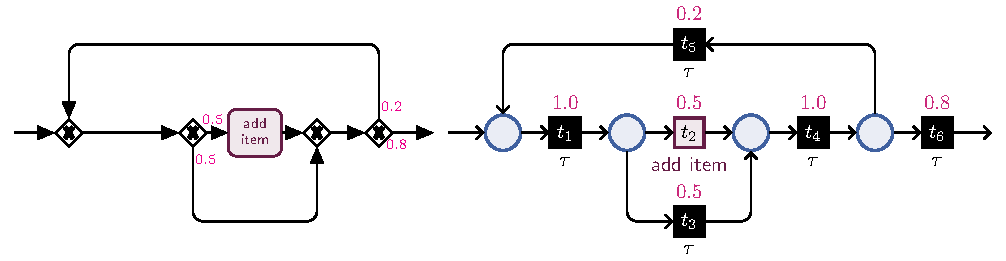
\includegraphics[width=\textwidth]{images/skip-iteration}
	\caption{A process model with a loop accepting fully silent iterations.}\label{fig:skip-iteration}
\end{figure}
\begin{figure}[!t]
		\centering
	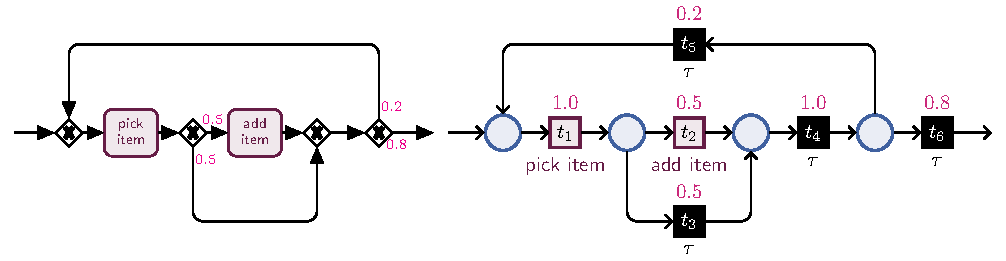
\includegraphics[width=\textwidth]{images/skip-step}
	\caption{A process model with a loop accepting iterations with skippable steps.}\label{fig:skip-step}
\end{figure}

\smallskip
\noindent
\textbf{Nets with ``bounded silence''.} The last requirement we impose over our nets is that of \emph{bounded silence}. This requirement states that the net cannot accept runs containing unboundedly many consecutive silent transitions. Mathematically, this means that there exists an a-priori bound on the maximum number of silent transitions that can be fired between two visible transitions. We comment on the suitability of this property in modeling terms, and on the advantage it gives when computing model trace probabilities.

In conceptual modeling terms, this requirement imposes that it is not possible to have loops in the process where an entire iteration consists only of visible transitions, that is, where an iteration can be executed without any visible task to witness its existence. We argue that, in this case, executing an entire iteration where all visible transitions are skipped is not different from the situation where the iteration is not executed at all. Consider, for example, the process fragment shown in Figure~\ref{fig:skip-iteration}. There, the trace consisting of three item additions could be produced by infinitely many distinct runs, each containing a different number of silent iterations in the loop.

On the other hand, it is perfectly possible to have loops with skippable tasks, provided that there exists at least one visible transition witnessing that an iteration in the loop has been executed. Figure~\ref{fig:skip-step} shows a variant of the process fragment in Figure~\ref{fig:skip-iteration} where each iteration must be witnessed by (visibly) picking an item, then deciding whether to add it or not (the latter choice resulting in a silent step). This variant has bounded silence, as two consecutive iterations need to contain two distinct executions of the \textsf{pick item} task, with at most one silent transition in between. 









 

\clearpage